\section{Modelling}

We can decouple worker applications from the front-end using asynchronous middleware.  Shared middleware balances the load, microservice architecture isolates it.  The system can adapt to current demand by using elastic scaling to create or destroy worker applications, and by using scaling groups we can ensure that the number of each application type is appropriate to the demand.

With care, we can use horizontal database partitioning to ensure that functions and/or data types are not shared between data nodes, isolating their demand from each other.

At the component level we can see whether an approach will balance or isolate load, or adapt to it, but at the system level we will need modelling techniques to predict the end to end throughput.

\paragraph{CloudSim.}  CloudSim \cite{calheiros2011cloudsim} is a Java framework for developing cloud datacentre simulations.  Much of it is concerned with modelling the efficient running of that infrastructure, for example the power usage, but it also includes utilisation models and may be useful for predicting the effect of elastic scaling.

CloudSim simulations require Java development for creation and modification, which is an overhead in building the models but offers more flexibility in applying them.  Process Algebra has closed-form solutions, though there is a PEPA Workbench tool \cite{gilmore1994pepa} that allows PEPA specifications to be parsed and run like programs, aiding experimentation on a range of action rates by automating repetitive calculations.  Both currently have their place as they predict different quantities of interest.

\paragraph{Process Algebra.} Process Algebras (such as PEPA or TIPP \cite{gotz1993multiprocessor}) allow us to model throughput in interdependent processes, with a mixture of independent and shared actions operating at different rates.  Each of our components can be described in this way, and queues have already been extensively modelled in PEPA \cite{thomas1997using}.  The nature of process algebra as a mathematical language also means that it is possible to build a model of a whole system by composition of the component models.

\begin{figure}
\caption{PEPA queue model}
\centering
% Automatically generated by PEPA2Latex
% --begin
\begin{displaymath}
	\begin{array}{rcl}
%[0.0ex]		
\mathit{Website} & \rmdef & (\mathit{request},\mathit{r}).\mathit{Website}\\
		\mathit{Worker} & \rmdef & (\mathit{service},\mathit{s}).\mathit{Worker}\\
		\mathit{Queue_{0}} & \rmdef & (\mathit{request},\mathit{r}).\mathit{Queue_{1}}\\
		\mathit{Queue_{1}} & \rmdef & (\mathit{service},\mathit{s}).\mathit{Queue_{0}}\\
[0.0ex]		\multicolumn{3}{l}{\mathit{Website}\sync{request}\mathit{Queue_{0}}[N]\sync{service}\mathit{Worker}}\\
[0.0ex]	\end{array}
\end{displaymath}
% --end
\end{figure}

%
% ---- PEPA Models
%

\section{PEPA Models}

%
% ---- Simple microservices
%
\subsection{Simple microservices}

\begin{figure}
	\caption{Simple microservices PEPA model}
	\centering
% --begin
\begin{displaymath}
	\begin{array}{rcl}
		\mathit{Website} & \rmdef & (\mathit{book\_athletics},\mathit{a}).\mathit{Website}+(\mathit{book\_cycling},\mathit{c}).\mathit{Website}\\
		\mathit{Athletics_{Worker}} & \rmdef & (\mathit{book\_athletics},\top).\mathit{Athletics_{Worker}}\\
		\mathit{Athletics_{DB}} & \rmdef & (\mathit{book\_athletics},\mathit{db\_a}).\mathit{Athletics_{DB}}\\
		\mathit{Cycling_{Worker}} & \rmdef & (\mathit{book\_cycling},\top).\mathit{Cycling_{Worker}}\\
		\mathit{Cycling_{DB}} & \rmdef & (\mathit{book\_cycling},\mathit{db\_c}).\mathit{Cycling_{DB}}\\
		[0.0ex]		\multicolumn{3}{l}{\mathit{Athletics_{Worker}}\sync{book\_athletics}\mathit{Website}\sync{book\_cycling}\mathit{Cycling_{Worker}}\sync{book\_athletics}\mathit{Athletics_{DB}}\sync{book\_cycling}\mathit{Cycling_{DB}}}\\
		[0.0ex]	\end{array}
\end{displaymath}
% --end
\end{figure}

\begin{figure}
	\caption{Simple microservices PEPA model - without worker processes}
	\centering
% --begin
\begin{displaymath}
\begin{array}{rcl}
		\mathit{Website} & \rmdef & (\mathit{book\_athletics},\mathit{a}).\mathit{Website}+(\mathit{book\_cycling},\mathit{c}).\mathit{Website}\\
\mathit{Athletics} & \rmdef & (\mathit{book\_athletics},\mathit{db\_a}).\mathit{Athletics}\\
\mathit{Cycling} & \rmdef & (\mathit{book\_cycling},\mathit{db\_c}).\mathit{Cycling}\\
[0.0ex]		\multicolumn{3}{l}{\mathit{Athletics}\sync{book\_athletics}\mathit{Website}\sync{book\_cycling}\mathit{Cycling}}\\
[0.0ex]	\end{array}
\end{displaymath}
% --end
\end{figure}

%
% ---- Operational microservices
%
\subsection{Operational microservices}



%
% ---- Shared queue middleware
%
\subsection{Shared queue middleware}

\begin{figure}
	\caption{Generic shared queue PEPA model}
	\centering
	% Automatically generated by PEPA2Latex
	% --begin
	\begin{displaymath}
		\begin{array}{rcl}
			\mathit{Arrival_1} & \rmdef & (\mathit{arrive_1},\mathit{a_1}).\mathit{Arrival_1}\\
			\mathit{Service_1} & \rmdef & (\mathit{serve_1},\mathit{s_1}).\mathit{Service_1}\\
			\mathit{Arrival_2} & \rmdef & (\mathit{arrive_2},\mathit{a_2}).\mathit{Arrival_2}\\
			\mathit{Service_2} & \rmdef & (\mathit{serve_2},\mathit{s_2}).\mathit{Service_2}\\
			\mathit{Q_0} & \rmdef & (\mathit{arrive_1},\top).\mathit{Q_1}+(\mathit{arrive_2},\top).\mathit{Q_1}\\
			\mathit{Q_1} & \rmdef & (\mathit{serve_1},\top).\mathit{Q_0}+(\mathit{serve_2},\top).\mathit{Q_0}\\
	[0.0ex]		\multicolumn{3}{l}{\mathit{Arrival_1}\sync{arrive_1}\mathit{Q_0}[N]\sync{serve_1}\mathit{Service_1}\sync{arrive_2}\mathit{Arrival_2}\sync{serve_2}\mathit{Service_2}}\\
	[0.0ex]	\end{array}
	\end{displaymath}
	% --end
\end{figure}

\begin{figure}
	\caption{Experimental results}
	\centering
	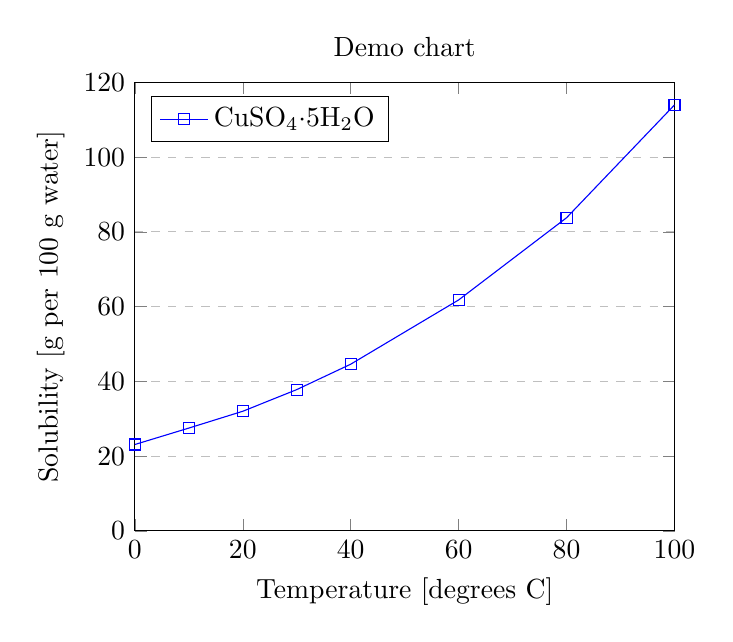
\begin{tikzpicture}
	\begin{axis}[
		title={Demo chart},
		xlabel={Temperature [degrees C]},
		ylabel={Solubility [g per 100 g water]},
		xmin=0, xmax=100,
		ymin=0, ymax=120,
		xtick={0,20,40,60,80,100},
		ytick={0,20,40,60,80,100,120},
		legend pos=north west,
		ymajorgrids=true,
		grid style=dashed,
	]
	
	\addplot[
		color=blue,
		mark=square,
		]
		coordinates {
			(0,23.1)(10,27.5)(20,32)(30,37.8)(40,44.6)(60,61.8)(80,83.8)(100,114)
		};
		\legend{CuSO$_4\cdot$5H$_2$O}
	
	\end{axis}
	\end{tikzpicture}
\end{figure}

\begin{figure}
	\caption{Application specific shared queue PEPA model}
	\centering
	% --begin
	\begin{displaymath}
	\begin{array}{rcl}
	\mathit{Website} & \rmdef & (\mathit{book\_athletics},\mathit{a}).\mathit{Website}+(\mathit{book\_cycling},\mathit{c}).\mathit{Website}\\
	\mathit{Athletics_{arrival}} & \rmdef & (\mathit{book\_athletics},\top).\mathit{Athletics_{arrival}}\\
	\mathit{Cycling_{arrival}} & \rmdef & (\mathit{book\_cycling},\top).\mathit{Cycling_{arrival}}\\
	\mathit{DBnode_1} & \rmdef & (\mathit{book\_athletics\_db},\mathit{db\_1}).\mathit{DBnode_1}\\
	\mathit{DBnode_2} & \rmdef & (\mathit{book\_cycling\_db},\mathit{db\_2}).\mathit{DBnode_2}\\
	\mathit{Q_{empty}} & \rmdef & (\mathit{book\_athletics},\top).\mathit{Q_{athletics}}+(\mathit{book\_cycling},\top).\mathit{Q_{cycling}}\\
	\mathit{Q_{athletics}} & \rmdef & (\mathit{book\_athletics\_db},\top).\mathit{Q_{empty}}\\
	\mathit{Q_{cycling}} & \rmdef & (\mathit{book\_cycling\_db},\top).\mathit{Q_{empty}}\\
	[0.0ex]		\multicolumn{3}{l}{\mathit{Website}\sync{book\_athletics,book\_cycling}\mathit{Athletics_{arrival}}\sync{book\_athletics}\mathit{Q_{empty}}[N]\sync{book\_athletics\_db}\mathit{DBnode_1}\sync{book\_cycling}\mathit{Cycling_{arrival}}\sync{book\_cycling\_db}\mathit{DBnode_2}}\\
	[0.0ex]	\end{array}
	\end{displaymath}
	% --end
\end{figure}

\begin{figure}
	\caption{Shared queue PEPA model without queue arrival processes}
	\centering
	% --begin
	\begin{displaymath}
	\begin{array}{rcl}
	\mathit{Website} & \rmdef & (\mathit{book\_athletics},\mathit{a}).\mathit{Website}+(\mathit{book\_cycling},\mathit{c}).\mathit{Website}\\
	\mathit{DBnode_1} & \rmdef & (\mathit{book\_athletics\_db},\mathit{db\_1}).\mathit{DBnode_1}\\
	\mathit{DBnode_2} & \rmdef & (\mathit{book\_cycling\_db},\mathit{db\_2}).\mathit{DBnode_2}\\
	\mathit{Q_{empty}} & \rmdef & (\mathit{book\_athletics},\top).\mathit{Q_{athletics}}+(\mathit{book\_cycling},\top).\mathit{Q_{cycling}}\\
	\mathit{Q_{athletics}} & \rmdef & (\mathit{book\_athletics\_db},\top).\mathit{Q_{empty}}\\
	\mathit{Q_{cycling}} & \rmdef & (\mathit{book\_cycling\_db},\top).\mathit{Q_{empty}}\\
	[0.0ex]		\multicolumn{3}{l}{\mathit{Website}\sync{book\_athletics,book\_cycling}\mathit{Q_{empty}}[N]\sync{book\_athletics\_db}\mathit{DBnode_1}\sync{book\_cycling\_db}\mathit{DBnode_2}}\\
	[0.0ex]	\end{array}
	\end{displaymath}
	% --end
\end{figure}

%
% ---- Distributed database with replication
%
\subsection{Distributed database with replication}

